%\documentstyle[epsf,twocolumn]{jarticle}       %LaTeX2e仕様
%\documentclass[twocolumn]{jarticle}     %pLaTeX2e仕様(platex.exeの場合)
\documentclass[onecolumn]{ujarticle}   %pLaTeX2e仕様(uplatex.exeの場合)
%%%%%%%%%%%%%%%%%%%%%%%%%%%%%%%%%%%%%%%%%%%%%%%%%%%%%%%%%%%%%%
%%
%%  基本バージョン
%%
%%%%%%%%%%%%%%%%%%%%%%%%%%%%%%%%%%%%%%%%%%%%%%%%%%%%%%%%%%%%%%%%
\setlength{\topmargin}{-45pt}
%\setlength{\oddsidemargin}{0cm}
\setlength{\oddsidemargin}{-7.5mm}
%\setlength{\evensidemargin}{0cm}
\setlength{\textheight}{24.1cm}
%setlength{\textheight}{25cm}
\setlength{\textwidth}{17.4cm}
%\setlength{\textwidth}{172mm}
\setlength{\columnsep}{11mm}

%\kanjiskip=.07zw plus.5pt minus.5pt


% 【節が変わるごとに (1.1)(1.2) … (2.1)(2.2) と数式番号をつけるとき】
%\makeatletter
%\renewcommand{\theequation}{%
%\thesection.\arabic{equation}} %\@addtoreset{equation}{section}
%\makeatother

%\renewcommand{\arraystretch}{0.95} 行間の設定
%%%%%%%%%%%%%%%%%%%%%%%%%%%%%%%%%%%%%%%%%%%%%%%%%%%%%%%%
%\usepackage{graphicx}   %pLaTeX2e仕様(\documentstyle ->\documentclass)
\usepackage[dvipdfmx]{graphicx}
\usepackage{subcaption}
\usepackage{multirow}
\usepackage{amsmath}
\usepackage{url}
\usepackage{ulem}
%%%%%%%%%%%%%%%%%%%%%%%%%%%%%%%%%%%%%%%%%%%%%%%%%%%%%%%%
\begin{document}

	%bibtex用の設定
	%\bibliographystyle{ujarticle}
	\noindent

	\hspace{1em}
	2019 年 12 月 27 日
	ゼミ資料
	\hfill
	M1 寺内 光

	\vspace{2mm}

	\hrule

	\begin{center}
		{\Large \bf 進捗報告}
	\end{center}


	\hrule
	\vspace{3mm}

	% ‚ここから 文章 Start!
	\section{今週やったこと}
	\begin{itemize}{
		\item{TensorFlowベースのdeeplabv3+のDocker化}
		\item{アノテーション改善して再学習}
		\item{Pytorchベースのdeeplabv3+に終止符を打った}
	}
	\end{itemize}

	\subsection{アノテーション改善した再学習}
	先々週,目と口のアノテーションを改善したのでそのデータセットで再学習.表 \ref{tab:touch_iou} に結果を示す.
	実験条件は後期発表会のものと同じである.萌えタッチの頬の部分を消したので萌えタッチの{\it mIoU}は下がったが,他の2タッチは主に口領域の分だけ {\it mIoU} が上がっている.
	全体としての{\it mIoU}も0.7%程向上している.

	\begin{table}[h]
		\centering
		\caption{改善前と改善後の{\it mIoU}}
		\label{tab:touch_iou}
		\begin{tabular}{|c||c|c|} \hline
			ジャンル&改善前&改善後\\ \hline
			訓練&0.7555&0.7609\\ \hline
			評価&0.6782&0.6859\\ \hline
			萌え&0.7224&0.7105\\ \hline
			青年&0.6559&0.6795\\ \hline
			少年&0.6388&0.6579\\ \hline
		\end{tabular}
	\end{table}

	また,図 \ref{fig:result} に改善前,改善後の検証画像に対する推論を示す.

	\begin{figure}[hb]
		\centering
		\begin{subfigure}{0.49\columnwidth}
			\centering
			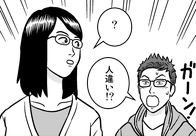
\includegraphics[width=1.0\columnwidth]{data/original_test_2.png}
				\caption{オリジナル画像(青年)}
		\end{subfigure}\\
		\begin{subfigure}{0.49\columnwidth}
			\centering
			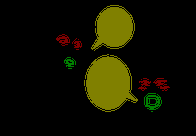
\includegraphics[width=1.0\columnwidth]{data/label_test_2.png}
				\caption{改善前ラベル画像}
		\end{subfigure}
		\begin{subfigure}{0.49\columnwidth}
			\centering
			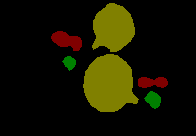
\includegraphics[width=1.0\columnwidth]{data/predict_test_2.png}
			\caption{改善前推論結果}
		\end{subfigure}
		\begin{subfigure}{0.49\columnwidth}
			\centering
			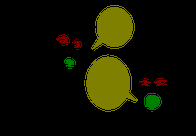
\includegraphics[width=1.0\columnwidth]{data/after_label.png}
				\caption{改善後ラベル画像}
		\end{subfigure}
		\begin{subfigure}{0.49\columnwidth}
			\centering
			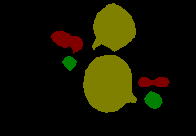
\includegraphics[width=1.0\columnwidth]{data/after_predict.png}
			\caption{改善後推論結果}
		\end{subfigure}
		\caption{検証画像 予測結果}
		\label{fig:result}
	\end{figure}


	\subsection{Pytorchベースのdeeplabv3+に終止符を打った}
	訓練済みモデルのシェイプ依存のところ以外を用いて再訓練したが,精度がほとんど変わらなかったので,ひとまずPyTorchベースのほうはおいておき,TensorFlowベースのものを使う.
	また,AutoDeepLabは沼が深そうだったので諦めた.

	\section{今後の方針}\noindent
	セマンティックセグメンテーションに関しては
	\begin{itemize}{
		\item{目のあたりのアノテーションをもう少しきれいに}
		\item{身体等別パーツを使う}
		\item{Manga109の漫画を推論する}
	}
	\end{itemize}
	等タスクとしては考えられる.

	今後はマルチモーダルでやりたいと思いつつ現状いい案があまり浮かばないので相談させてください.

\end{document}
